\documentclass[nobib]{tufte-handout}

\title{Lecture 7: The max-flow min-cut theorem $\cdot$ 1MA020}

\author[Vilhelm Agdur]{Vilhelm Agdur\thanks{\href{mailto:vilhelm.agdur@math.uu.se}{\nolinkurl{vilhelm.agdur@math.uu.se}}}}

\date{14 November 2023}


%\geometry{showframe} % display margins for debugging page layout

\usepackage{graphicx} % allow embedded images
  \setkeys{Gin}{width=\linewidth,totalheight=\textheight,keepaspectratio}
  \graphicspath{{graphics/}} % set of paths to search for images
\usepackage{amsmath}  % extended mathematics
\usepackage{booktabs} % book-quality tables
\usepackage{units}    % non-stacked fractions and better unit spacing
\usepackage{multicol} % multiple column layout facilities
\usepackage{lipsum}   % filler text
\usepackage{fancyvrb} % extended verbatim environments
  \fvset{fontsize=\normalsize}% default font size for fancy-verbatim environments

\usepackage{color,soul} % Highlights for text

% Standardize command font styles and environments
\newcommand{\doccmd}[1]{\texttt{\textbackslash#1}}% command name -- adds backslash automatically
\newcommand{\docopt}[1]{\ensuremath{\langle}\textrm{\textit{#1}}\ensuremath{\rangle}}% optional command argument
\newcommand{\docarg}[1]{\textrm{\textit{#1}}}% (required) command argument
\newcommand{\docenv}[1]{\textsf{#1}}% environment name
\newcommand{\docpkg}[1]{\texttt{#1}}% package name
\newcommand{\doccls}[1]{\texttt{#1}}% document class name
\newcommand{\docclsopt}[1]{\texttt{#1}}% document class option name
\newenvironment{docspec}{\begin{quote}\noindent}{\end{quote}}% command specification environment

\include{mathcommands.extratex}

\begin{document}

\maketitle% this prints the handout title, author, and date

\begin{abstract}
\noindent
Continuing our exploration of things that can be done with weighted graphs, we move on to considering \emph{flows} in weighted directed graphs, which model things like traffic flows. We see the connection between these and edge cuts of graphs, and prove the Ford-Fulkerson theorem.
\end{abstract}

In our exercises, we saw this figure:
\begin{figure}
    \centering
    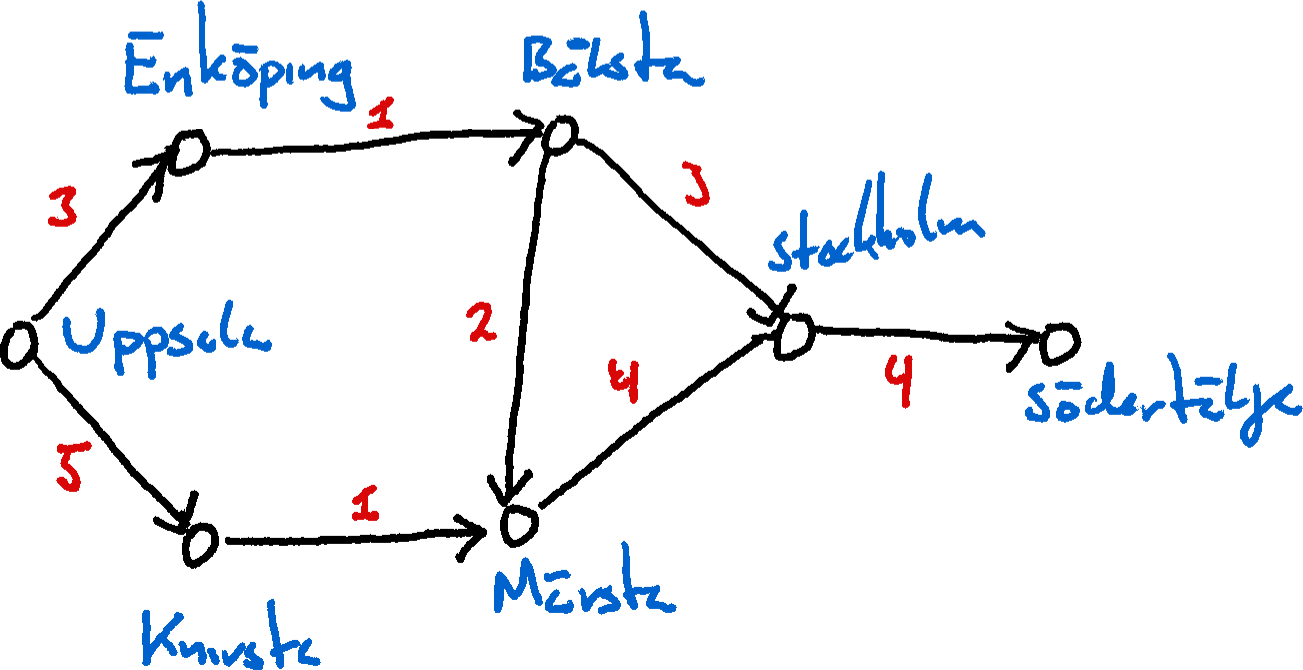
\includegraphics[width=0.85\textwidth]{graphics/L5_exc_MSTs_etc/train_network_flow.png}
    \caption[][0cm]{A hypothetical graph modelling public transport flow from Uppsala to Södertälje.}
    \label{fig:uppsala_stockholm_traffic}
  \end{figure}

  If we interpret the edge-weights as how many thousands of passengers can travel the route per hour, it makes sense to ask the question of how many can travel from Uppsala to Södertälje per hour. Intuitively, it is clear that the answer must be two thousand, because the traffic is bottlenecked by the Enköping-Bålsta and Knivsta-Märsta connections -- the fact that five thousand per hour can get from Uppsala to Knivsta doesn't help at all, and upgrading the Bålsta-Stockholm route wouldn't improve things.

  Let us now turn these intuitive considerations into actual rigorous mathematics. First, let us define the graphs we are working on:

  \begin{definition}
    A \emph{weighted directed graph} $G$ consists of a directed graph $(V,E)$ and a weight function $w: E \to \R$. For it to be a \emph{flow network} we additionally require that all weights be positive, that there be a distinguished \emph{source} vertex $s$ and \emph{sink} vertex $t$, and that whenever $u \to v$ is an edge, $v \to u$ is not also an edge.\sidenote[][-3cm]{Recall that in general, it is allowed in a simple directed graph to have both the edge $u\to v$ and the edge $v\to u$ -- what is not allowed is multiples of the same edge, or loops. In this case, the restriction of not having such back-and-forth edges is not a genuine restriction, however: If we have such a pair of edges, we can get an equivalent flow network by introducing a ``dummy vertex'' in the middle of one of the edges, as in Figure \ref{fig:dummy_edge}.}

    \begin{marginfigure}
        \centering
        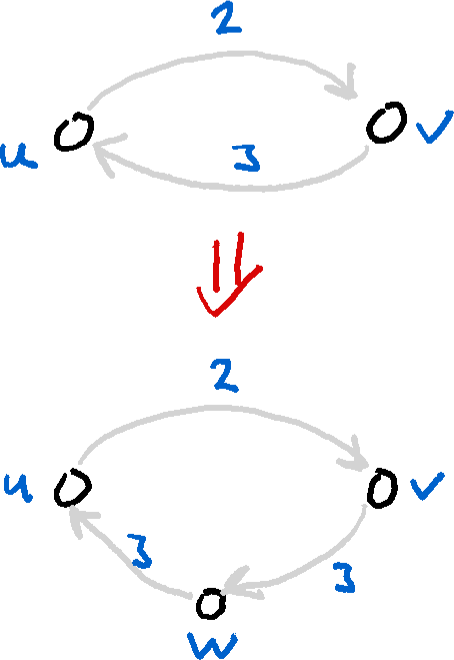
\includegraphics[width=0.5\textwidth]{graphics/L7_flows/dummy_edge.png}
        \caption{Subdividing an edge using a dummy vertex, to get around the restriction that there be no back-and-forth edges.}
        \label{fig:dummy_edge}
    \end{marginfigure}

    We define a \emph{capacity function} $c: V\times V \to [0,\infty)$ by that $c(v,v') = w(v\to v')$ whenever $v\to v'$ is an edge of $G$, and $c(v,v') = 0$ otherwise.
  \end{definition}

  These flow graphs define the capacity of the network to handle traffic. Next, let us define the actual \emph{flows}, which are the possible actual traffic situations. There are two natural constraints these should satisfy:
  \begin{enumerate}
    \item The flow through an edge can't be greater than the actual capacity of the edge, so we aren't putting more cars on the road than will actually fit.
    \item Other than the source and the sink nodes, where we imagine vehicles are entering and exiting the graph, the flow into a vertex must equal the flow out of it. Trains do not magically vanish, nor do they appear out of nowhere or teleport.
  \end{enumerate}

  \begin{definition}
    A \emph{flow} on the flow network $G$ with capacity function $c$ is a function $f: V \times V \to [0,\infty)$ which satisfies
    \begin{enumerate}
        \item the \emph{capacity constraint} that
        $$f(v, v') \leq c(v, v')\qquad \forall v, v' \in V,$$
        \item and the \emph{conservation constraint}
        $$\sum_{w \in V} f(w, x) = \sum_{u \in V} f(x, u)$$
        whenever $v \in V \setminus \{s,t\}$.
    \end{enumerate}
  \end{definition}




\section{Exercises}

%\bibliography{references}
%\bibliographystyle{plainnat}

\end{document}
